\subsection{بخش چ}
در این بخش به بررسی اثر بیشترین نرخ چرخش قابل مشاهده جست‌وجوگر بر فاصله‌ ازدست‌دهی پرداخته شده است.
\begin{figure}[H]
	\centering
	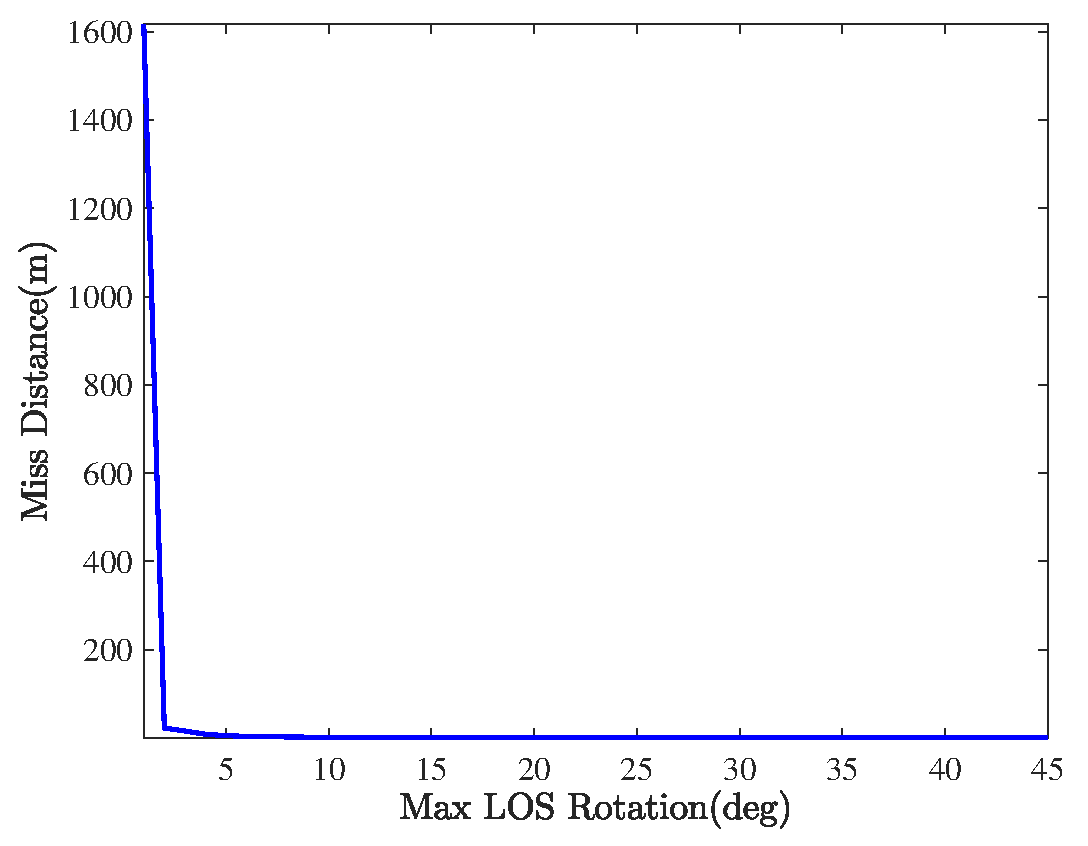
\includegraphics[width=.75\linewidth]{../Figure/Q1/g/MD}
	\caption{فاصله ازدست‌دهی برای مقادیر مختلف بیشترین نرخ چرخش قابل مشاهده}
\end{figure}
بر اساس نتایج شبیه‌سازی، هر چه بیشترین نرخ چرخش بالا برود، فاصله ازدست‌دهی کاهش می‌یابد. مقدار قابل قبول متناسب با هدف انتخاب می‌شود. بر اساس نتایج شبیه‌سازی در نرخ چرخش ۵ درجه مقدار فاصله ازدست‌دهی کم و بیشترین نرخ چرخش معقول است.